\documentclass[11pt]{article}

\usepackage[hyphens]{url}

\usepackage[document]{ragged2e}

\usepackage{hyperref}
\hypersetup
{
    breaklinks = true,
    allcolors = black,
    linktoc = all
}

\usepackage{mathtools}
\usepackage{amssymb}
\usepackage{stmaryrd}
\usepackage{graphicx}

\usepackage{multicol}
\setlength{\columnseprule}{0.4pt}

\usepackage{listings}
\lstloadlanguages{Haskell}
\lstset
{
    basicstyle=\small\ttfamily,
    flexiblecolumns=false,
    basewidth={0.5em,0.45em},
    literate={+}{{$+$}}1 {/}{{$/$}}1 {*}{{$*$}}1 {=}{{$=$}}1
            {>}{{$>$}}1 {<}{{$<$}}1 {\\}{{$\lambda$}}1
            {\\\\}{{\char`\\\char`\\}}1
            {->}{{$\rightarrow$}}2 {>=}{{$\geq$}}2 {<-}{{$\leftarrow$}}2
            {<=}{{$\leq$}}2 {=>}{{$\Rightarrow$}}2 
            {\ .}{{$\circ$}}2 {\ .\ }{{$\circ$}}2
            {>>}{{>>}}2 {>>=}{{>>=}}2
            {|}{{$\mid$}}1 {\$}{\$}1         
}

\usepackage[english]{babel}
\usepackage[utf8]{inputenc}
\usepackage{fancyhdr}
\pagestyle{fancy}
\fancyhf{}
\rhead{James Burton}
\lhead{ID: 4251529}
\fancyfoot[C]{\thepage}

\usepackage{titling}
\title
{ 
    \vspace{10em}
    G53IDS - Final Report \\
    \hfill \break
    \large Embedded Domain Specific Language for \\
    Describing Recipes in Haskell
}

\setlength{\droptitle}{-10em}

\author{James Burton - 4251529 - psyjb6}

\begin{document}
\maketitle
\newpage

% Abstract and Acknowledgements
% 4 sentence abstract
% State the problem
% Why it's an interesting problem
% What my solution achieves
% What follows from my solution

\newpage

\tableofcontents
\newpage

\section{Introduction and Motivation}
\subsection{Overview}
Consider the following recipe to make a cup of tea:
\begin{tt}
\small
\begin{lstlisting}
    - Boil some water
    - Pour over a teabag
    - Wait for 5 minutes
    - Remove the teabag
    - Add milk (optional)
\end{lstlisting}
\end{tt}

This is a very simple but useful recipe that many people
will perform, in some cases, many times a day over their lives.
What we can realise by looking at this recipe is that it actually
consists of many smaller recipes, such as boiling water and
combining tea with milk, performed in a certain order. This
raises the question, to what extent does the order matter and
to what extent can we rearrange things in order to make the recipe
more efficient? No doubt you have done this, maybe subconsciously,
while cooking at home. Furthermore which steps can be done
concurrently in the event that multiple people are cooking e.g.
in a professional kitchen with a full brigade?

\medbreak

Perhaps closer to computer science, we could also ask, how could
we instruct a robot to do this? After doing some research on
robotic chefs it appears that not a huge number exist.
There is one home cooking robot \cite{robot} which uses motion
capture in order to learn recipes. In my opinion this is rather
restrictive. It presumes that the human performs the recipe in
the optimal manner and it would be very difficult to model
a brigade system in this way. In reality there is a limited set
of fundamental actions that one becomes able to perform when
learning to cook. Recipes can then be performed using a sequence
of these actions. Representing recipes like this would allow us
to take a robot programmed to perform each of the fundamental
actions and tell it how to cook literally anything. This is the
same principle as taking code written in a high level language
and compiling it down into a sequence of low level actions in
assembly language.

\medbreak

What is needed is a consistent way of representing recipes to
a computer such that they can be manipulated in various ways
for example scheduling, calculation of cost or even generating
suggestions on how to improve the recipe. My contributions
to solving this problem are the following:

\begin{itemize}
    \item I have provided a set of combinators as an EDSL in Haskell and show that
    they can be used to describe a wide variety of recipes (Section 2).

    \item I have defined a set of actions needed to actually execute a recipe (Section 3).

    \item I have defined what it means for two recipes to be equal.

    \item I have scheduled recipes defined in the EDSL using a representation
    of a kitchen environment. The schedule is optimised based on the tree-like
    structure of recipes in the EDSL.
\end{itemize}

\subsection{DSLs and Haskell}
Domain Specific Languages (DSLs) are programming languages that
are designed for use in a certain problem domain rather than
being general purpose. As such they trade range of expression
for clarity of expression. A frequently used example of a DSL
is the popular database querying language, SQL.

\medbreak

Embedded Domain Specific Languages (EDSLs) are DSLs that are embedded
within another language, such as Haskell. This allows for
fast development as you no longer need to write your parser
or compiler; programs written in your EDSL can just be interpretted
as programs written using the language in which it is embedded.
Secondly it allows programs written in your language to be
manipulated using the full power of the host language. Taking
an example from this project, if recipes were specified as a DSL
then in order to schedule them, one would have to either expand
the DSL to handle scheduling or write something in another language
to interpret the recipes so that they can be scheduled. In this
case the recipe EDSL is in Haskell and as such a scheduler can
just be written in Haskell as it would for any other purpose thus
saving both time and unecessary extra code.

\medbreak

Haskell is a very popular language for writing EDSLs, examples
range from pretty printing \cite{pretty} to financial contracts \cite{contracts}.
Reasons for this include that the type checker catches many mistakes
and that Haskell has very lightweight function application syntax
allowing us to omit symbols such as brackets in many cases \cite{snoyman}.

\subsection{Deep and Shallow Embedding}
When writing an EDSL one must choose between deep and shallow embedding.
Deep embedding means that the DSL's abstract syntax tree (AST) is
represented using an algebraic data type. On the other hand, shallow
embedding doesn't have an AST and the language constructs exist purely
as mappings to their semantics.

\medbreak

Both of these approaches have their advantages. Deep embedding
allows us to transform the representation before evaluating
it however, every time we want to add a new language construct
then we need to add it to the AST and as such our data type
can become quite large. Similarly, all functions manipulating
the AST must be changed to accomodate the new construct. Shallow
embedding avoids these issues as it doesn't have an AST however,
it does mean that we are limited to a specific semantic domain.

\medbreak

For the recipe DSL I have decided to borrow some features from
both. The fundamental actions which compose a recipe use a
deep embedding allowing us to evaluate the recipes in multiple
semantic domains for example cost or time. The functions
exposed to the user represent more of a shallow embedding
which makes the definition of recipes much more concise and
means that any new combinator can be added trivially as long
as it can be represented as some construction of the deeply
embedded actions.

\section{Combinators}
\subsection{Initial Definitions}


\subsection{Sequencing Problem}
\subsection{Conditionals}
\subsection{Transactions}
\subsection{Moving to a Tree of Actions}
\subsection{Final Definitions}
\subsection{Custom Combinators}

\section{Deriving Equality}
In this section I shall discuss what it means for two recipes
to be equal and how that has been used with QuickSpec \cite{quickspec, quickspec2}
in order to find algebraic properties held by recipes.

\subsection{Topological Sorting}
When considering what it means for two recipes to be equal one
might consider that they must have the same ingredients
and the same actions must be performed on those ingredients,
in the same order.

\medbreak

Our recipe tree already encodes the ingredients and the actions
performed on them, they are nodes in the tree. Ordering of
actions in our tree is captured by their level in the tree.
We can see that the actions we could choose to perform first
are the leaves of the tree. If we then remove a leaf and perform
that action then the actions we can perform next are the new
leaves of the tree. We can use this to generate a list of all
the different orders that the actions of a recipe can be performed
in while creating the same recipe. We want a way of generating
all combinations of nodes such that nodes higher in the tree
appear after their children in the list thus preserving the
order of our actions.

\medbreak

This is known as topological sorting. I have implemented a
function in Haskell below which, given a recipe, returns a list
of all topological sorts of that recipe.

\begin{lstlisting}
    topologicals :: Recipe -> [[Action]]
    topologicals (Node a []) = [[a]]
    topologicals t = concat
        [map (a:) (topologicals' l) | l@(Node a _) <- ls]
        where
            topologicals' l = topologicals $ removeFrom t l
            ls = leaves t
\end{lstlisting}

As an example, consider this alternate definition for our
cup of tea recipe. 

\begin{lstlisting}
    cupOfTea' :: Recipe
    cupOfTea' = optional $ combine "mix" 
        ( removeAfter (minutes 5)
        $ combine "mix" teabag
        $ heatTo 100 water ) milk
\end{lstlisting}

In this version we combine our tea with milk rather than combing milk with our tea.
Printing the trees for this recipe gives a different result from our original recipe.

\begin{figure}[h]
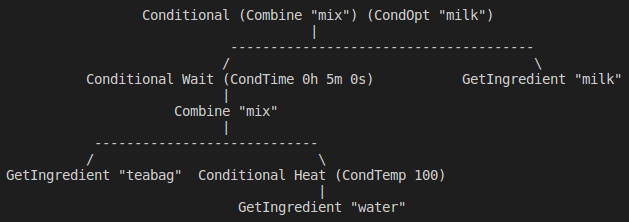
\includegraphics[width=\textwidth, keepaspectratio]{cupOfTea2.png}
\centering
\caption{Alternate cup of tea recipe printed as a tree.}
\end{figure}

In Haskell one must make their data type an instance of the \texttt{Eq} typeclass in
order to make use of the \texttt{==} operator. The equality instance for recipes is
defined as follows.

\begin{lstlisting}
    instance {-# OVERLAPPING #-} Eq Recipe where
        (==) r1 r2 = let xs = sort $ topologicals r1
                         ys = sort $ topologicals r2
                      in xs == ys
\end{lstlisting}

Because \texttt{Recipe = Tree Action} it naturally uses the equality instance for
\texttt{Tree} but we want to use our topological sorting. That's what the "overlapping"
annotation is for. As for the actual definition, we are simply taking the topological sorts
of each recipe, sorting them and then checking if those two lists are equal. If they are
then our recipes are equal. Using the above definition, the expression \texttt{cupOfTea == cupOfTea'}
evaluates to \texttt{True} showing that, as desired, our two recipes are equal.

\medbreak

As a side note \texttt{sort} requires an instance of \texttt{Ord} which means that values have some
natural order. This isn't defined for \texttt{Tree} by default and as such I have defined it as follows.

\begin{lstlisting}
    instance Eq a => Ord (Tree a) where
        compare t1 t2 = compare (length t1) (length t2)
\end{lstlisting}

This simply compares trees based on their length i.e.
their number of nodes.

\subsection{Quickspec}

\section{Scheduling Recipes}

Now that we have a solid representation of our recipes in Haskell we can think about how
these could be scheduled.

\subsection{Modelling a Kitchen}

The first step of scheduling a recipe is to consider some representation of the
environment within which it is scheduled. Abstracting from the details we can
break a kitchen down into a set of stations for example an oven and a kettle.
We also need some sort of global observables for example, time.

\begin{lstlisting}
    data Env = Env
        { eStations :: [Station]
        , eObs      :: [IO Obs]
        }

    data Station = Station
        { stName     :: String
        , stConstrF  :: ConstraintF
        , stObs      :: [IO Obs]
        }

    type ConstraintF = Recipe -> Maybe [Process]
\end{lstlisting}

Stations consist of a name, a constraint function and a set of local observables such as temperature.
The constraint function takes a recipe and returns a list of processes required to perform that recipe.
In the event that the station cannot handle that particular recipe then \texttt{Nothing} is returned.
A process is an intermediate translation of our recipes. One might say it's our sort of assembly
language, sitting between our high level combinators and some device specific instructions that the
developer of a robot chef might write.

\begin{lstlisting}
    data Process =
        Input
        | Output
        | Preheat Int
        | DoNothing
        | PCombine String
        | EvalCond Condition
        | MeasureOut Measurement
\end{lstlisting}

Most of these are self explanatory, \texttt{PCombine} and \texttt{MeasureOut} are just renamings of
the actions \texttt{Combine} and \texttt{Measure}. \texttt{EvalCond} is inserted after \texttt{Input}
which when interpreted will check the condition, if true then skip to \texttt{Output} else it will
run all processes up until \texttt{Output} before jumping back to the condition again. As an example
the following part of our cup of tea recipe:

\begin{lstlisting}
    Conditional (CondTemp 100) Heat ->
        [Input, EvalCond (CondTemp 100), Output]
\end{lstlisting}

The water is put into the kettle which then heats it until the temperature is 100 degrees
before the water is taken out. You might be wondering why there is no "heat" process.
That's because something is heated as a side effect of being placed in a device which becomes hot
rather than as an explicit action of that device. Device specific details such as the kettle turning
on when the water is added or turning off on output is not covered here as these details can
be abstracted away being \texttt{Input} and \texttt{Output}.

\subsection{Scheduling Methods}

Now that we have a model of a cooking environment we need to choose a method for scheduling the recipes.
Scheduling is in itself a complex problem and therefore the solution used for this project is by
now means suggested as a well refined solution but merely a demonstration of using the recipe system
for a more concrete purpose.

\subsubsection{Linear Programming}
The first consideration was linear programming (LP). LP works by taking a linear function, called
the objective function, which is minimised or maximised according to a set of linear constraints.
For our recipes the objective function would be the end time of the final step which we would then
want to minimise in order to make the recipe as efficient as possible. We then might consider the
following constraints.

\[ end_r = start_r + dur_r \quad \forall r \]

\[ start_r \geq end_d \quad \forall d,r \quad | \quad d \in dependencies(r) \]

That is the end time of each recipe is equal to its start time plus its duration and a recipe
must start at or after the end time of its dependencies.

The problem arose with choosing which station to schedule each action on. For any action we
have a set of stations that can perform that action. We can then expand our first constraint
to handle this.

\[ end_{r_s} = start_{r_s} + dur_{r_s} \quad \forall r,s \quad | \quad s \in validStations(r) \]

But we only want one of the valid stations to be selected which leaves us with the problem
of modelling logical OR in this context. One potential way is to use a set of binary variables
as follows.

\[ end_r = \sum (end_{r_s} * bin_{r_s}) \quad \forall r,s \quad | \quad s \in validStations(r) \]

\[ \sum_{s}^{validStations(r)} end_{r_s} = 1 \quad \forall r \]

The issue with the above is that it involves the multiplication of two variables. As such this
is no longer a linear constraint. A long time was spent considering whether or not our recipes
could in fact be expressed as linear systems. After reformulating the problem several times
and not finding a solution I decided to move on from linear programming and find something else.

\subsubsection{Bin Packing}

Bin packing is a much more general optimisation problem. It is the problem of packing a number
of objects with fixed dimensions into a number of bins of fixed dimensions such that the number
of bins is minimised. This problem as it is doesn't bare much resemblance to our recipes however,
adjusting the problem as follows provides something more useful.

\medbreak

Given a number of objects of fixed height and a number of bins of infinite height where each
bin can only hold certain types of object. Pack the objects into the bins such that the
height of the tallest stack is minimised and a set of constraints regarding order of
objects is met. We can model our stations as a stack of actions which they must perform,
these are our bins. Our objects are either the station performing one of our actions
or being idle for a certain time. We can then say that the height an action begins on
the stack must be greater than or equal to the height that its dependencies end on their
respective stacks.

\medbreak

As an abstract example, imagine a recipe, r1, which has sub-recipes: r2, r3 and r4. All the
recipes must be scheduled on station 2, except r3 which must be scheduled on station 1.
Below is a diagram showing r1 and a potential stack setup.

\begin{figure}[h]
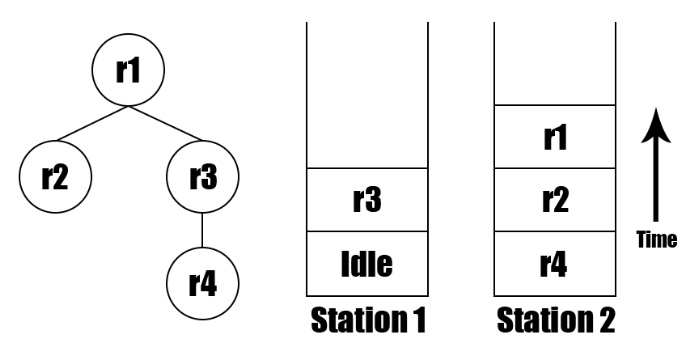
\includegraphics[width=10cm, keepaspectratio]{stacks.png}
\centering
\caption{Recipe tree and stack schedule for r1.}
\end{figure}

\subsection{Optimisations and Heuristics}

Now that we have a way to translate our recipes into a form of schedule we need to consider
optimisations we can apply during the scheduling process. As mentioned in the introduction,
you have no doubt done this while cooking at home. In the case of making a cup of tea you
may start the kettle boiling before you get the milk out of the fridge. That way, you and
the kettle are working in parallel and thus saving time.

\medbreak

Heuristics are "rules of thumb" that are applied to a problem solver in order to guide it
in the decision making process. An everyday example might be preferring motorways over country roads
when planning a journey; they have a higher speed limit and traffic capacity thus making
them a faster route in the general case. There are two decisions we can apply heuristics to
when scheduling recipes. The first is which leaf of the recipe tree to schedule first.
Referring back to the section on topological sorting, the leaves of the tree at a given time
are comprise the set of actions we can choose to perform next. The second decision is which
of the available stations to schedule this action on.

\subsubsection{Leaf Choice Heuristics}

The first heuristic used in leaf choice is "shortest task first". This may seem counter intuitive however,
if we think about the way in which recipes are typically structured, it makes sense. It is frequent
to have a small task such as "get water" followed by a longer task performed by another station
for example "boil water". Let's say that "get milk" was a long task to complete. It would make more
sense to do the short "get water" task first, start the kettle boiling, then use that time to
"get milk". If we "get milk" first then we're performing a long task, meanwhile the kettle is idle
waiting for some water.

\medbreak

The second heuristic is applied in the event that multiple leaves contain a task of the shortest length.
It is based on the same principle as above, that if we have short task such as "get water" followed
by a lengthy task such as "boil water" we want to "get water" as soon as possible so that the kettle
can be boiling while we do the other tasks. This is formalised as "longest branch first". In the
event that there are multiple "shortest tasks" then the task on the longest branch will be chosen
to try and ensure that if we have a long task that depends on a short task, it will be started
as soon as possible.

\subsubsection{Stack Choice Heuristics}

Now that we have selected which leaf to schedule, we need to choose which station to schedule it on.
In many cases this is a simple task as many actions can only be performed by one station. In the event
that multiple stations can be used then we use three heuristics to choose, each shortening the list of
potential stations.

\medbreak

The first is to pick whichever station is in least demand. This is done by scanning through all unscheduled
actions and calculating their time divided by the number of stations that action could be performed on.
For example if an action a had a time of 10 and could be performed on either of 2 stations then the demand
that a would create for each station would be 5. The reason for this heuristic is rather intuitive. If we
have a choice between a station which a lot of other actions need and a relatively uneeded station, we should
choose the uneeded station to reduce the load on the high demand station. This heuristic could obviously
be inverted if the goal was to minimise stations used rather than time taken.

\medbreak

The second heuristic is "least idle time". One's first thought might be to add the action to the emptiest
stack however, in the event that the action is waiting on a long dependency, it could cause lots of idle
time to be added to an otherwise empty stack. Therefore we choose the stack which allows the action to be
started closest to the end time of its dependencies which may mean placing it on a fuller stack rather than
an emptier one.

\medbreak

It is unlikely that the first two heuristics didn't filter the potential stations down to one, but if they
didn't then we select the stack that is least full. Providing there are no caveats like idle time, as mentioned
above, then placing an action on an emptier stack should result in a shorter overall time in most cases.

\subsection{Implementation}

For the sake of space, I shalln't go into the details of the code here as there is quite a lot of it
However, below is some pseudo-code to demonstrate the general flow of the scheduling functions.

\begin{lstlisting}
    data Task = Active Label | Idle Time

    type Stack = [Task]

    type Schedule = Map StName Stack

    schedule :: Recipe -> Env -> Schedule
    schedule r env = do
        tree = labelRecipe r
        schedule' env tree tree emptySch
        where
            schedule' env fullTree tree sch = do
                l = chooseLeaf tree
                st = chooseStation fullTree l env sch
                stack = lookup st sch
                stack' = Active l : stack
                newSch = insert st stack' sch
                if l == root fullTree
                    then
                        newSch
                    else
                        tree' = removeFrom tree l
                        schedule' env fullTree tree' newSch
\end{lstlisting}

The main function \texttt{schedule} takes a recipe and an environment then returns a schedule.
It first labels the recipe, this is to avoid issues with a set of actions appearing on multiple
branches. It then passes the environment, two copies of the recipe tree and an empty initial
schedule to the sub-routine \texttt{schedule'}. The reason for passing two copies of the tree
is that one is maintained as the full tree in order to maintain access to the children of the
node we are scheduling even after those child nodes have been scheduled and removed from the other
tree. The functions \texttt{chooseLeaf} and \texttt{chooseStation} apply the various heuristics
and return the best leaf and best station respectively. Next we add the leaf to the stack of
the chosen station and update the schedule. We then check to see if the node we just
scheduled is the root of the tree, if it then we have finished and can return our new schedule
otherwise we pass our new schedule and updated tree to the next iteration of \texttt{schedule'}.

\subsection{Cold Toast}

This method of scheduling seems to work however, there is one problem that arises from us
reordering steps in order to optimise them. Consider the following recipe for tea and buttered toast,
for conciseness I have omitted the ingredient definitions.

\begin{lstlisting}
    cupOfTea :: Recipe
    cupOfTea = optional $ combine "mix" milk
        $ waitFor (minutes 5)
        $ combine "mix" teabag
        $ heatTo 100 water

    butteredToast :: Recipe
    butteredToast = combine "spread" butter
        $ heatFor (minutes 3) bread

    teaWithToast :: Recipe
    teaWithToast = combine "place next to"
        butteredToast
        cupOfTea
\end{lstlisting}

It could be the case that, when scheduling, first the bread is toasting, then the cup of tea is
made, then the butter is added to the toast. The problem with this is that by the time we come
to spread the butter on the toast, it has gone cold. We need some way to ensure that the butter
is added immediately after the toast is finished. To do this we have a new combinator called
\texttt{Transaction} which wraps any other action. This can then be interpretted by the scheduling
function to mean that the action which it wraps and it's immediate children should be scheduled
together meaning that no other actions can end up in between. Our buttered toast recipe is now
as follows.

\begin{lstlisting}
    butteredToast :: Recipe
    butteredToast = transaction
        $ combine "spread" butter
        $ heatFor (minutes 3) bread
\end{lstlisting}

\section{Recipe Properties}
\subsection{Folding Over Recipes}
\subsection{Time and Cost}
\subsection{Generating Recipes}
\subsection{Improving Recipes}

\section{Development Process}
\subsection{Project Management}
\subsection{Evaluation and Testing}
\subsection{Test Recipes}
\subsection{QuickCheck}

\section{Summary and Reflections}
\subsection{Project Management}
\subsection{Contributions}
\subsection{Future Work}
\subsection{Reflections}

\section{Related Work}
\subsection{Pretty Printing}
\subsection{Financial Contracts}
\subsection{Deep vs Shallow Embedding}
\subsection{Regions}
\newpage

    \begin{thebibliography}{8}

        \bibitem{robot}
        The Guardian. 2015. \textit{Future of food: how we cook}.
        \url{https://www.theguardian.com/technology/2015/sep/13/future-of-food-how-we-cook}
        Online. Accessed April 2, 2018.

        \bibitem{hudak}
        Paul Hudak. Domain Specific Languages. Department of Computer
        Science, Yale University, December 15, 1997.

        \bibitem{snoyman}
        Michael Snoynman. O'Reilly Webcast: Designing Domain Specific
        Languages with Haskell. January 4, 2013.
        \url{https://www.youtube.com/watch?v=8k_SU1t50M8}
        Online. Accessed April 2, 2018.

        \bibitem{contracts}
        Simon Peyton Jones, Microsoft Research, Cambridge.
        Jean-Marc Eber, LexiFi Technologies, Paris. Julian Seward,
        University of Glasgow. Composing contracts: an adventure in
        financial engineering. August 17, 2000.

        \bibitem{pretty}
        John Hughes. The Design of a Pretty-printing Library.
        Chalmers Teniska Hogskola, Goteborg, Sweden. 1995.

        \bibitem{embedding}
        Josef Svenningsson. Emil Axelsson. Combining Deep and Shallow
        Embedding of Domain-Specific Languages. Chalmers University
        of Technology. February 27, 2015.

        \bibitem{contracts-pp}
        Simon Peyton Jones, Microsoft Research, Cambridge.
        Jean-Marc Eber, LexiFi Technologies, Paris. Julian Seward,
        University of Glasgow. Composing contracts: an adventure in
        financial engineering (PowerPoint Slides). August 17, 2000.
        \url{https://www.microsoft.com/en-us/research/publication/composing-contracts-an-adventure-in-financial-engineering/}

        \bibitem{core}
        Simon Peyton Jones. Into the Core - Squeezing Haskell into
        Nine Constructors. September 14, 2016.
        \url{https://www.youtube.com/watch?v=uR_VzYxvbxg}
        Online. Accessed April 2, 2018.

        \bibitem{hutton-fold}
        Graham Hutton. Fold and Unfold for Program Semantics. Department of
        Computer Science, University of Nottingham. September 1998.

        \bibitem{quickspec}
        Koen Claessen, Chalmers University of Technology. Nicholas Smallbone,
        Chalmers University of Technology. John Hughes, Chalmers and Quviq AB.
        QuickSpec: Guessing Formal Specifications using Testing.
        September 28, 2013.

        \bibitem{quickspec2}
        Nicholas Smallbone. Moa Johansson. Koen Claessen. Maximilian Algehed.
        Chalmers University of Technology.
        Quick Specifications for the Busy Programmer. January 31, 2017.

    \end{thebibliography}   

    \newpage

    \appendix

\end{document}